\documentclass{article}


\usepackage{amsmath,amssymb,graphicx,amsthm,xparse, color, mathrsfs} 
\usepackage{ epstopdf, fullpage}

\newcommand{\showsolution}[1]{\textbf{Ans.}\;#1}


\newcommand{\minimize}[1]{\underset{#1}{\mathrm{minimize}}}
\newcommand{\argmin}[1]{\underset{#1}{\mathrm{argmin}}}
\newcommand{\argmax}[1]{\underset{#1}{\mathrm{argmax}}}
\newcommand{\st}{\text{subject to}}
\newcommand{\rank}{\textbf{rank}}
\newcommand{\diag}{\textbf{diag}}
\newcommand{\mb}{\mathbf}
\newcommand{\tr}{\mathbf{tr}}
\newcommand{\mL}{\mathcal L}
\newcommand{\mC}{\mathcal C}
\newcommand{\mP}{\mathcal P}
\newcommand{\mN}{\mathcal N}
\newcommand{\mZ}{\mathcal Z}

\newcommand{\proj}{\mathbf{proj}}
\newcommand{\vnull}{\mathbf{null}}
\newcommand{\range}{\mathbf{range}}
\renewcommand{\Re}{\mathbf R}
\newcommand{\red}[1]{{\color{red}#1}}
\newcommand{\bmat}{\left[\begin{matrix}}
\newcommand{\emat}{\end{matrix}\right]}





\newcommand{\mypagebreak}{\begin{center}\noindent\makebox[\linewidth]{\rule{7.5in}{1pt}} \end{center}}

\begin{document}
	{\Large\textbf{CPSC 406: Homework 1}}



\begin{enumerate}
	
	\item \textbf{Backsolve} Here, we will explore the computational complexity of solving the system 
	\[
	Rx = b, \qquad R\in \Re^{n\times n}
	\]
	when $R$ is either upper triangular ($R_{ij} = 0$ whenever $i > j$) or lower triangular ($R_{ij} = 0$ whenever $i < j$). If $R$ were fully dense, then solving this system takes $O(n^3)$ flops. We will show that when $R$ is upper or lower triangular, this system takes $O(n^2)$ flops. Assume that the diagonal elements $|R_{ii}| > \epsilon$ for $\epsilon$ suitably large in all cases.


	\begin{enumerate}
		\item Consider $R$ lower triangular, e.g. we solve the system
		\[
		\bmat 
		R_{11} & 0 & \cdots & 0 \\
		R_{21} & R_{22} & \cdots & 0 \\
		\vdots  & \vdots  & \ddots & \vdots  \\
		R_{n,1} & R_{n,2} & \cdots & R_{n,n}\\
		\emat 
		\bmat x_1 \\ x_2 \\ \vdots \\ x_n \emat 
		=
		\bmat b_1 \\ b_2 \\ \vdots \\ b_n \emat. 
		\]
		Show how to find $x_1$. (This should take $O(1)$ flops.)  Given $x_1,...,x_i$, show how to find $x_{i+1}$. (This should take $O(i)$ flops.) Putting it all together, we get 
		\[
		O(1) + O(2) + \cdots + O(n-1) + O(n) = O(n^2) \text{ flops.}
		\]
		
		\showsolution{
		\[
		x_1 = b_1/R_{11}, \quad x_{i+1} = \frac{b_{i+1} - \sum_{k=1}^i R_{i+1,k}x_k}{R_{i+1,i+1}}.
		\]	
		}
		\item Now consider $R$ upper triangular, e.g. we solve the system
		\[
		\bmat 
		R_{11} &  \cdots & R_{1,n-1} &R_{1,n} \\
		 0     &  \cdots & R_{2,n-1} &R_{2,n} \\
		\vdots  & \ddots    &  \vdots &\vdots  \\
		0 &  \cdots & 0 &R_{n,n}\\
		\emat 
		\bmat x_1 \\ x_2 \\ \vdots \\ x_n \emat 
		=
		\bmat b_1 \\ b_2 \\ \vdots \\ b_n \emat. 
		\]
		Show how to find $x_n$. (This should take $O(1)$ flops.)  Given $x_{i+1},...,x_n$, show how to find $x_{i}$. (This should take $O(n-i)$ flops.) Putting it all together, we get 
		\[
		O(n) + O(n-1) + \cdots + O(2) + O(1) = O(n^2) \text{ flops.}
		\]
		
		\showsolution{
			\[
			x_n = b_n/R_{nn}, \quad x_{i} = \frac{b_{i} - \sum_{k=i+1}^n R_{i,k}x_k}{R_{i,i}}.
			\]	
		}
	\end{enumerate}

\item \textbf{Linear data fit} Download \red{data}. Fit the best line 
\[
f(z) = x_1 + x_2z 
\]
to the points $(z_1,y_1),...,(z_n,y_n)$; that is, find the best approximation of the line $f(z)$ to $y$ in the 2-norm sense.
Plot the fit, and report $\|r\|_2$ the norm of the fit residual.

\showsolution{
\begin{center}
	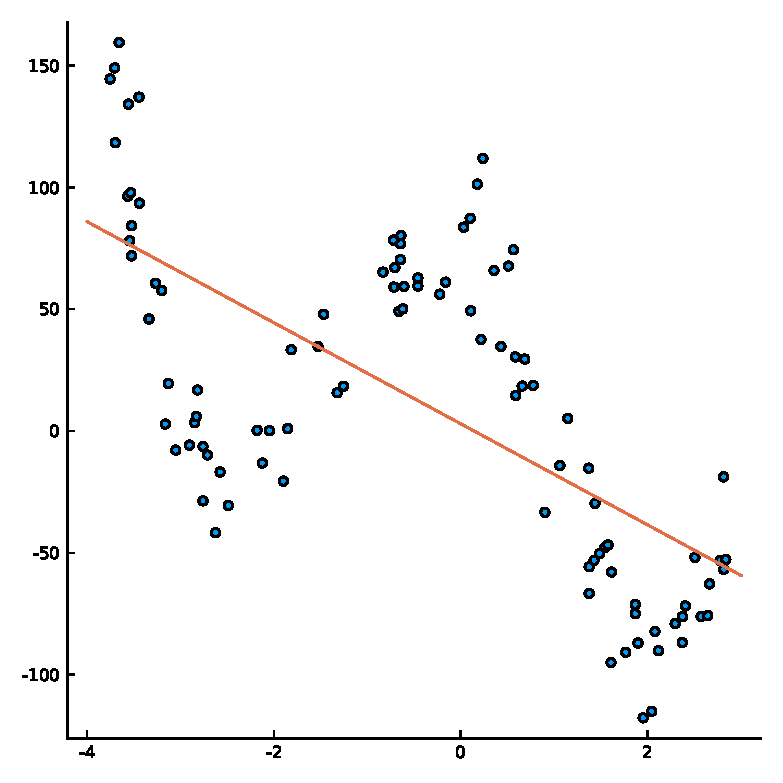
\includegraphics[width=3in]{img/hw1_p2_o1.eps}
\end{center}
residual $\|b-Ax\|_2 = 498.56$
}

\item \textbf{Polynomial data fit}  Using the same data as above, fit the best order-$d$ polynomial to the points $(z_1,y_1),...,(z_n,y_n)$ , for $d = 2,3,4,5$. That is, find $x_1,...,x_{d+1}$ such that 
\[
f(z) = x_1 + x_2z + x_3z^2 + \cdots + x_{d+1}z^d
\]
best approximates the data in the 2-norm sense (minimizing $\sum_i (f(z_i)-y_i)^2$).
Plot the fit, and report $\|r\|_2$ the norm of the fit residual. About how many degrees is needed for a reasonable fit?

\showsolution{
	\begin{center}
		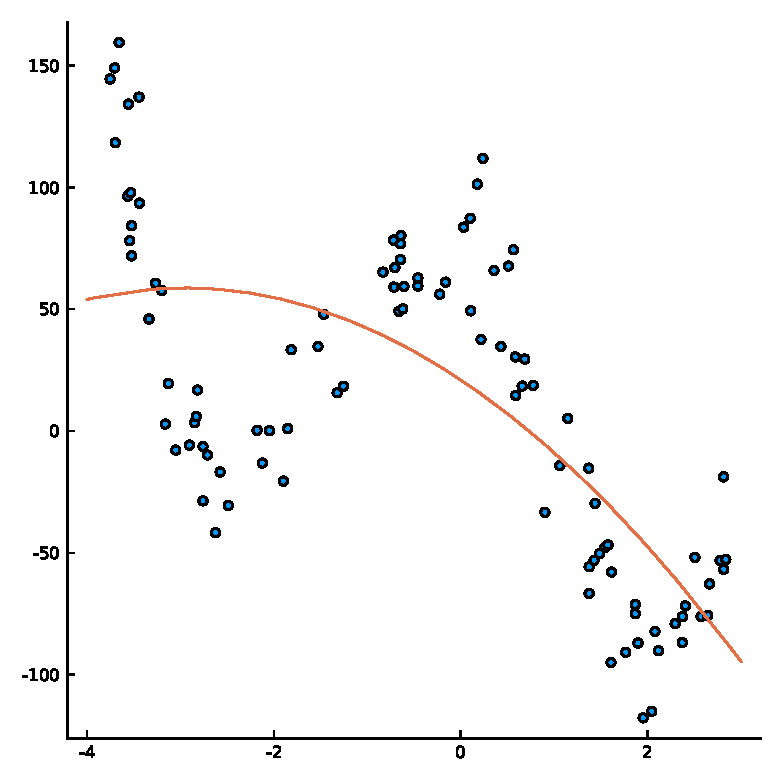
\includegraphics[width=3in]{img/hw1_p2_o2.eps}
		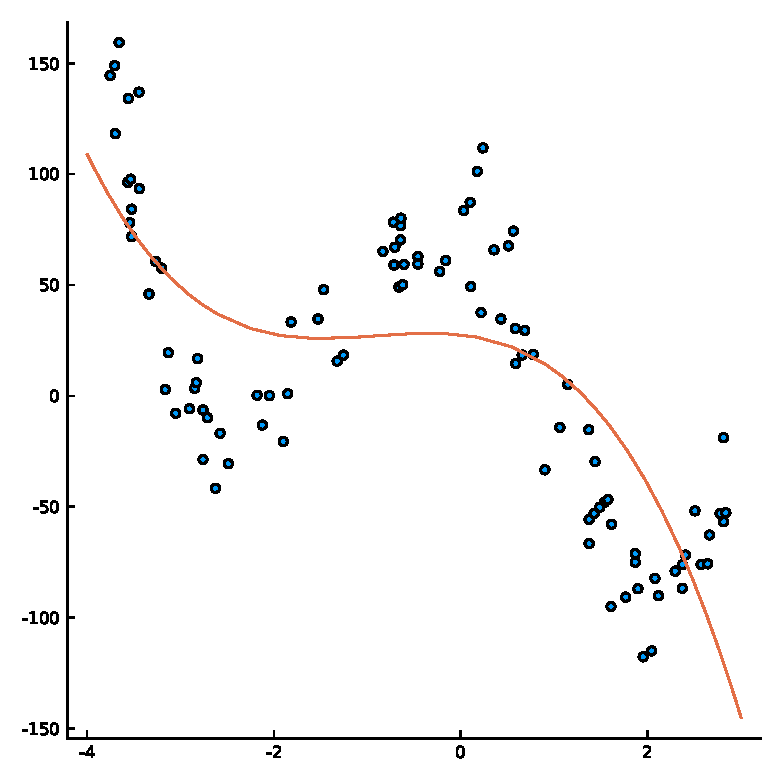
\includegraphics[width=3in]{img/hw1_p2_o3.eps}
		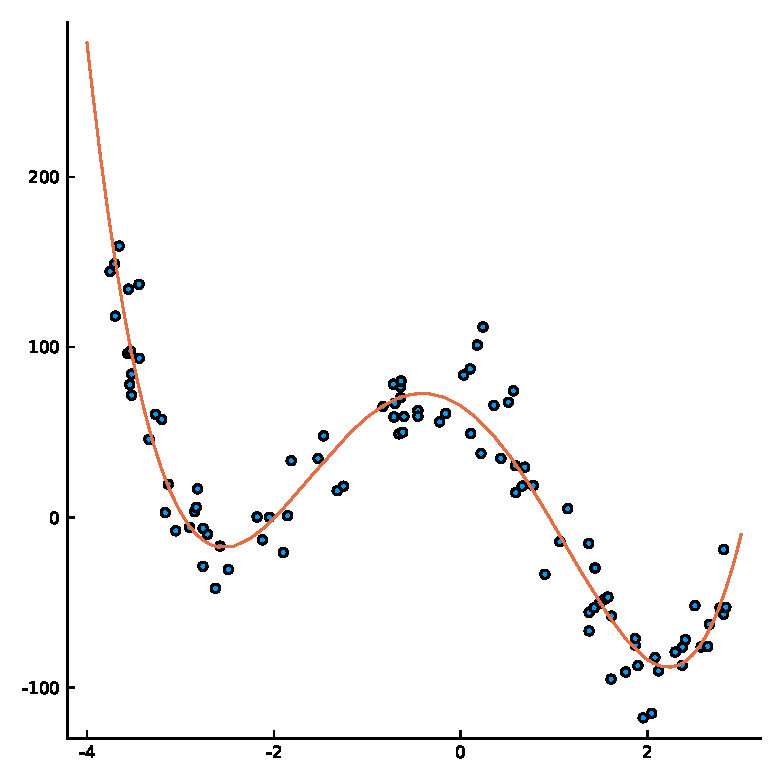
\includegraphics[width=3in]{img/hw1_p2_o4.eps}
		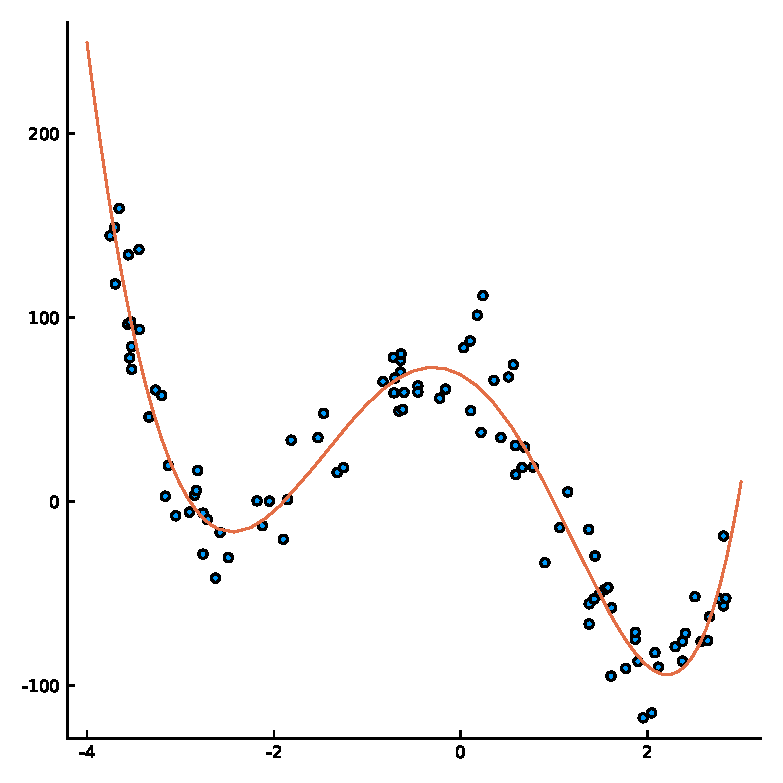
\includegraphics[width=3in]{img/hw1_p2_o5.eps}
	\end{center}
	residuals:
	\begin{itemize}
		\item $d=2,\|b-Ax\|_2 = 473.93$
		\item $d=3,\|b-Ax\|_2 = 439.14$
		\item $d=4,\|b-Ax\|_2 = 194.79$
		\item $d=5,\|b-Ax\|_2 = 189.05$
	\end{itemize}
You see a sharp improvement at $d = 4$, but $d = 5$ doesn't really add much, so $d=4$ is needed for a reasonable fit.
}

\item Consider the full rank, underdetermined but consistent linear system $Ax = b$, where $A$ is $m\times n$ with $m < n$. 
 \begin{enumerate}
	\item Show how to use the QR factorization to obtain a soution of this system.
	
 	\showsolution{
There are two ways we can factor $A$. If we factor as $A = QR$, we get something like
\[
\underbrace{\bmat 
\times  & \times & \times & \times & \times& \times \\
\times  & \times & \times & \times & \times & \times\\
\times  & \times & \times & \times & \times & \times\\
\times  & \times & \times & \times & \times & \times
\emat 
}_{A}
=
\underbrace{\bmat 
\times  & \times & \times & \times  \\
\times  & \times & \times & \times  \\
\times  & \times & \times & \times  \\
\times  & \times & \times & \times  \\
\emat }_{Q}
\underbrace{\bmat 
\times  & \times 	& \times & \times & \times & \times\\
0  		& \times 	& \times & \times & \times & \times\\
0  		& 0		 	& \times & \times & \times& \times \\
0  		& 0		 	& 0 & \times & \times & \times
\emat }_{R}
\]
and we can solve 
\[
x = R^{-1}Q^Tb.
\]
The key advantage is that $Q$ is only $m\times m$, and $R$ is the same storage as $A$, so the only increase in storage is $m^2$. But, inverting $R$ is tricky, as it is not exactly triangular.

We can also factor $A^T=QR$ to get something like
\[
\underbrace{\bmat 
	\times  & \times & \times & \times  \\
	\times  & \times & \times & \times \\
	\times  & \times & \times & \times \\
	\times  & \times & \times & \times \\
	\times  & \times & \times & \times \\
	\times  & \times & \times & \times 	
	\emat 
}_{A^T}
=
\underbrace{\bmat 
	\times  & \times & \times & \times  \\
	\times  & \times & \times & \times \\
	\times  & \times & \times & \times \\
	\times  & \times & \times & \times \\
	\times  & \times & \times & \times \\
	\times  & \times & \times & \times 	
	\emat }_{Q}
\underbrace{\bmat 
	\times  & \times & \times & \times  \\
	0  & \times & \times & \times \\
	0  & 0 & \times & \times \\
	0  & 0 & 0 & \times 
	\emat. }_{R}
\]

Overall, we will solve this system in two steps:
\[
 R^Tz = b, \quad Q^Tx = z.
\]
The first step is now much easier. 
When $R$ is wide, it is tricky to figure out how to invert it. But when $R$ is square, it is easy to ``invert" through backsolving. 

The second step is tricky, because $Q^T$ is wide, and not easily left invertible. In fact, there are many solutions for $x$. One possible solution is 
$x = QQ^Tz$, which is the least squares solution, and perhaps easiest to compute in this context. 

In this regime, the solve system $z = R^{-T}b$ takes $O(m^2)$ flops, and $x = Qz$ requires $O(mn)$ flops, for a total of $O(mn+m^2)$ flops for the solve, and an extra $O(nm^2)$ flops for the original QR factorization.
}
	\item The following script can be used to generate random matrices in Julia, given dimensions $m$ and $n$:
	
	\begin{verbatim}
	A = randn(m,n);
	x = randn(n,1);
	b = A*x;
	\end{verbatim}
	
	Write Julia code for solving for $x$ using the procedure outlined in the previous part of the question. Record the runtime
	 using the Julia call \texttt{time}. (Make sure you are not running anything else or it will interfere with the timing 
	 results.) Record the runtimes for matrices of sizes  $(m,n) = (10,20)$, $(100,200)$, $(100,2000)$,  $(100,20000)$, and 
	 $(100,200000)$. Compare the runtimes against finding $x$ using \verb|x = A\b|.
	
	
	\showsolution{
		Here's some simple code:
		
		\texttt{\~{}, t1 = @timed begin\\
        F = qr(A') \\
        x1 = F.Q*(F.R'$\backslash$b)\\
    	end\\ \newline
    	\~{}, t2 = @timed begin\\
        x2 = A$\backslash$b \\
		end\\}   
	
		
		On my personal laptop, in seconds
		
		\begin{tabular}{|l|ccccc|}
			\hline
			$(m,n)$ &  $(10,20)$& $(100,200)$& $(100,2000)$&  $(100,20000)$ & $(100,200000)$\\
			\hline
			QR				& 0.00005 & 0.0012 & 0.0076 & 0.0654 & 0.7892\\
			$A\backslash b$	& 0.00005 & 0.0020 & 0.0327 & 0.3377 & 4.8510\\
			\hline
		\end{tabular}
	
		}

\end{enumerate}



\end{enumerate}
\begin{thebibliography}{1}
	
	\bibitem{beck2014introduction}
	{\sc A.~Beck}, {\em Introduction to nonlinear optimization: theory, algorithms,
		and applications with MATLAB}, vol.~19, Siam, 2014.
	
\end{thebibliography}

\end{document}